\documentclass[12pt,a4paper]{article}
\usepackage{lipsum}
\usepackage{authblk}
\usepackage{graphicx}
\usepackage[top=2cm, bottom=2cm, left=2cm, right=2cm]{geometry}
\usepackage{fancyhdr}
%
\pagestyle{fancy}
%
\renewenvironment{abstract}{%
\hfill\begin{minipage}{0.95\textwidth}
\rule{\textwidth}{1pt}}
{\par\noindent\rule{\textwidth}{1pt}\end{minipage}}
%
\makeatletter
\renewcommand\@maketitle{%
\hfill
\begin{minipage}{0.95\textwidth}
\vskip 2em
\let\footnote\thanks 
{\LARGE \@title \par }
\vskip 1.5em
{\large \@author \par}
\end{minipage}
\vskip 1em \par
}
\makeatother
%
\begin{document}
%
%title and author details
\title{Architect short tutorial}
\author[1]{SPARC\_Lab}
\affil[1]{00044, Italy, Frascat(RM), via E.Fermi, LNF INFN}
%
\maketitle
%
\begin{abstract}
This tutorial provides a short instruction on how to install the Architect on the Windows-PC and basic information on how to use it. 
\end{abstract}
\section*{What You will need}

In order to use Architect on Win You will need two things:
\begin{itemize}
\item{CygWin}
\item{GitHub}
\end{itemize}

I do believe those programs can be substituted with something else. For example GitHub is needed only to down load the architect itself and keep up with updates. In addition to that You might want to install some kind of a .txt editor for work with input Architect files (e.g. PSPad).
\section{CygWin}
In order to install CygWin You will need a setup file - google it. At start of the setup You will be asked about the server from which will be download the CygWin itself - pick any, it does not matter. CygWin has a lot of packages (see. Fig.\ref{fig1}) and You certainty don't need all of them. In order to make Architect work You will need to install only \textit{Base} and \textit{Devel}.

\begin{figure}[h]
\centering
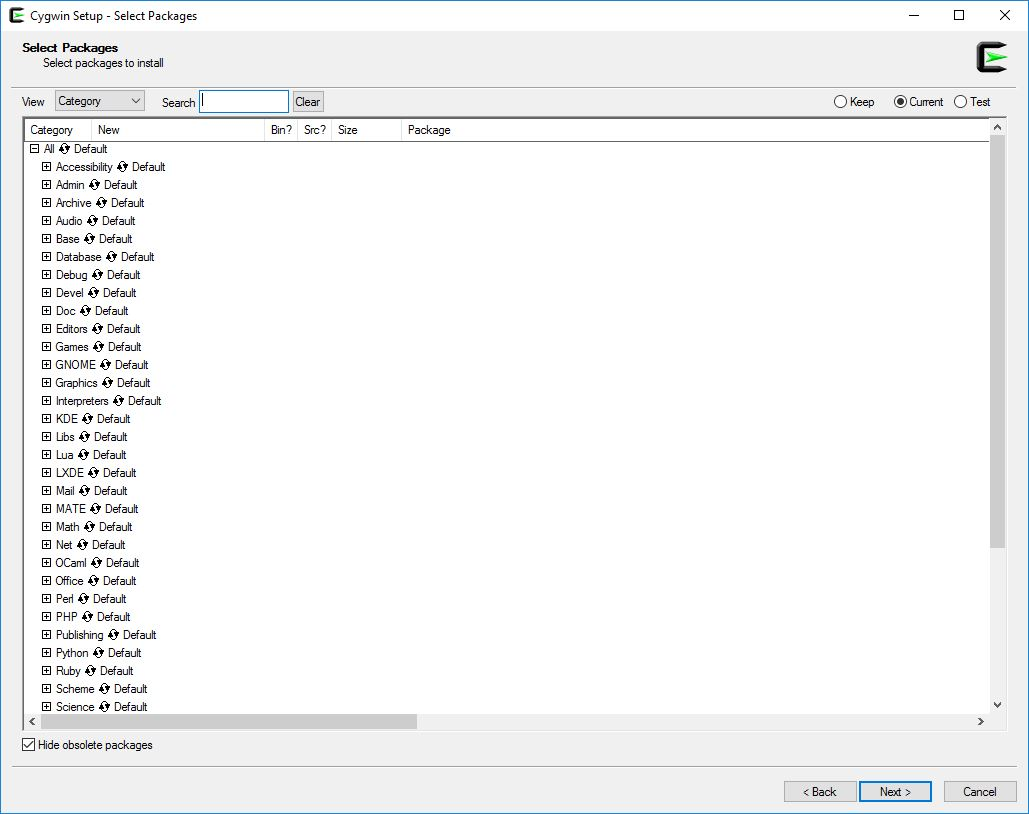
\includegraphics[width=0.6\textwidth]{CygWin_Packages.jpg}
\caption{Cygwin packages. You will need only \textit{Base} and \textit{Devel}.}
\label{fig1}
\end{figure}
It will take some time to install everything, but this is it with CygWin installation.

\section{GitHub}
Now You will need to download the Architect files. It can be done from GitHub repository, so You will need GitHub itself. Again the GitHub setup file can be googled. After You will install the GitHub go to GitHub.com and register/sign up to You account and find Architect repository (see Fig.\ref{fig2}). Click "Clone or download" and clone Architect into Your CygWin installation folder "...\textbackslash cygwin64\textbackslash home". That is it, after that You will need only update from time to time Your Architect from GitHub.

\begin{figure}[h]
\centering
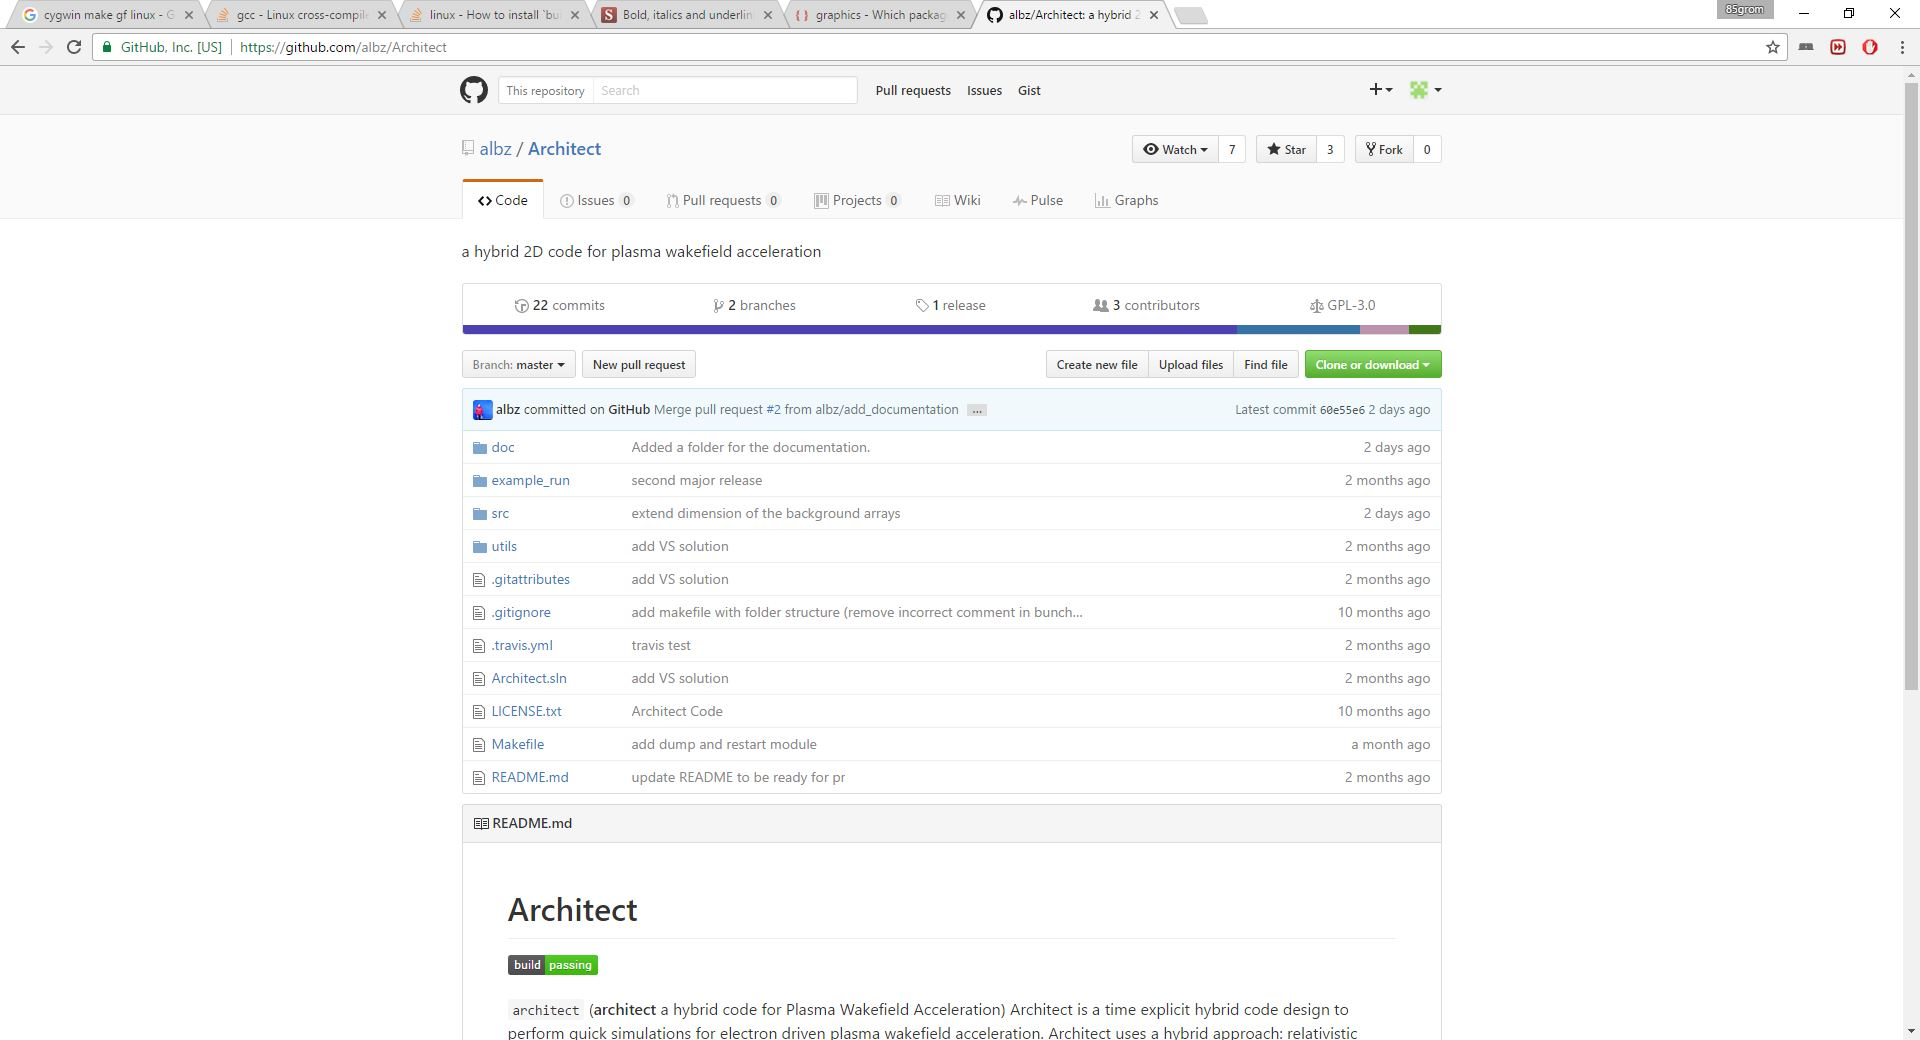
\includegraphics[width=0.6\textwidth]{GitHub_web_Architect.jpg}
\caption{Architect at GitHub web cite.}
\label{fig2}
\end{figure}

\section{How to actually run it}

Well, start up the CygWin and go to Your home Architect folder (see Fig.\ref{fig3}). Then using command \textit{make gflinux} generate .exe file that will be stored in "...\textbackslash cygwin64\textbackslash home\textbackslash Architect\textbackslash bin". Now You can go to the folder in Architect directory that called "example\_run" where You will find file "architect.nml". This is a name list where You set the parameters of Your simulations. In order to run it You just need, being inside the folder with this file, indicate where is Your Architect.exe file, thus it will be something like: "..\textbackslash bin\textbackslash Architect.exe". This will start the simulation and create a number of output folders inside the "..\textbackslash example\_run". That it is, You started the Architect simulation.

\begin{figure}[h]
\centering
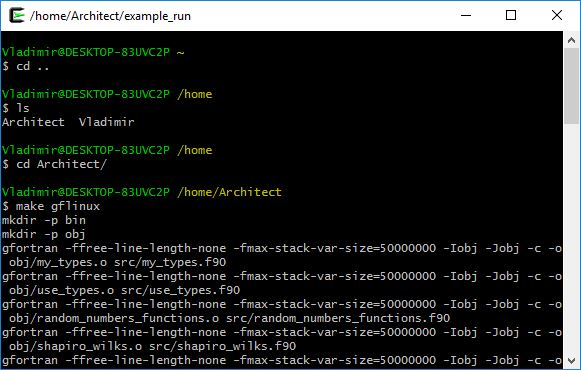
\includegraphics[width=0.6\textwidth]{CygWin_make_file.jpg}
\caption{How to make .exe file for Architect.}
\label{fig3}
\end{figure}

\section{Name List}
Name list, as the name suggests, contains the parameters of the simulation (see Fig.\ref{fig4}). Last time when I used Architect ( a couple of month ago) I had a different template for the name list, thus I will be able to give comments on very few lines in .nml file. Luckily a lot of strings have comments and lot of variables have transparent names.
\begin{figure}[h]
\centering
\includegraphics[width=0.6\textwidth]{Name_list_PSPad.jpg}
\caption{"Example\_run" name list in PSPad.}
\label{fig4}
\end{figure}

Here is the description of some of the strings: 
\begin{itemize}
\item{\textit{plasma\%l\_acc=30050.0} 

String number 3.Length of the plasma. Parameter is given in $\mu m$.}
\item{\textit{plasma\%n0=1.0e16}

String number 6. Plasma density in $cm^{-3}$.}
\item{\textit{bunch\_initialization\%n\_total\_bunches=2} 

String number 123. Total number of bunches in the simulation.}

\item{\textit{bunch\_initialization\%db(1)=0.,} 

String number 130. Point where the centroid of the first bunch is originally placed. If I am not mistaken this parameter always should be 0.}

\item{\textit{bunch\_initialization\%db(2)=0.45,} 

String number 131. Point where the centroid of the second bunch is originally placed. The position of the bunch is given in terms of plasma wavelength $\lambda_p$, meaning that every time when You change plasma density You change the absolute position of the second beam with respect to the first bunch.}

\item{\textit{bunch\_initialization\%ChargeB(1)=0.200,}

\textit{bunch\_initialization\%ChargeB(2)=0.060,} 

Strings number 133 and 134, correspondingly. Charge of the first and second bunches, can be more. The number of those bunches is defined by the "total\_bunches" parameter.}

\item{\textit{bunch\_initialization\%shape(1)=1,}

\textit{bunch\_initialization\%shape(2)=1,} 

Strings number 136 and 148, correspondingly. If remember this correctly this is the longitudinal profile of the bunches and "1" is the Gaussian distribution.}


\item{\textit{bunch\_initialization\%n\_particles(1)=100000,}

\textit{bunch\_initialization\%n\_particles(2)=50000,} 

Strings number 137 and 149, correspondingly. The number of (macro?)particles that considered inside the bunch. The more the better, but slower.}

\item{\textit{bunch\_initialization\%bunch\_s\_x(1)=4.0,}

\textit{bunch\_initialization\%bunch\_s\_y(1)=4.0,}

\textit{bunch\_initialization\%bunch\_s\_z(1)=50.0,}

\

\textit{bunch\_initialization\%bunch\_s\_x(2)=4.0,}

\textit{bunch\_initialization\%bunch\_s\_y(2)=4.0,}

\textit{bunch\_initialization\%bunch\_s\_z(2)=50.0,} 

Strings number 138-140 and 150-152, correspondingly. The size of the beam in x,y,z directions. I do believe that for normal distribution beam those are $\sigma$'s.}

\item{\textit{bunch\_initialization\%bunch\_gamma\_m(1)=200.,}

\textit{bunch\_initialization\%bunch\_dgamma(1)=0.100,}

\

\textit{bunch\_initialization\%bunch\_gamma\_m(2)=200.,}

\textit{bunch\_initialization\%bunch\_dgamma(2)=0.100,}

Strings number 141,144 and 153,156, correspondingly. Initial energy of the bunches and energy spread. Energy is given in terms of Lorentz factor. The energy spread is given as $\Delta\gamma/\gamma$.}

\item{\textit{Osys\%macwin=1} 

String number 199. This parameter defines the OS You work with, since this tutorial mostly for Windows family, this parameter should be "1".}

\item{\textit{bck\_plasma\%order\_radial(1)=0,}

\textit{bck\_plasma\%order\_radial(2)=0,}

This parameter set the profile of the background plasma. Following values of this parameter can be applied:

	\begin{itemize}
	\item{0: Uniform density in \_r\_}
	\item{3: The profile starts from a fixed value at r=0 and decays with a cos$<$sup$>$2$<$/sup$>$ shape reaching zero  at \_r\_=**radius\textbackslash\_um**.}
	\item{4: The profile has a cos$<$sup$>$2$<$/sup$>$ shape shrunk vertically by a factor **perturbation\textbackslash\_amplitude** and shifted upwards by a **certain value**. The 	profile drops to 0 with a step at \_r\_=**radius\textbackslash\_um**}
	\item{5: The profile has a flat-top with a **certain hight** from \textbackslash\_r\textbackslash\_=0 to 

	r=**radius\textbackslash\_internal\textbackslash\_um** then, from **radius\textbackslash\_internal\textbackslash\_um** to **radius\textbackslash\_um** the 		profile 		decays with a cos$<$sup$>$2$<$/sup$>$ shape. }
	\end{itemize}
}
\end{itemize}



\section{Useful MatLab utilities}

In order to process the Architect data there are several useful scripts that can be found in Architect files (something like ...\textbackslash Architect\textbackslash utils\textbackslash MatLab\_utils). The easiest way to use those scripts is to add them into MatLab command library. Just click "Set\_folder" and choose the folder with Architect utilities.
\begin{figure}[h]
\centering
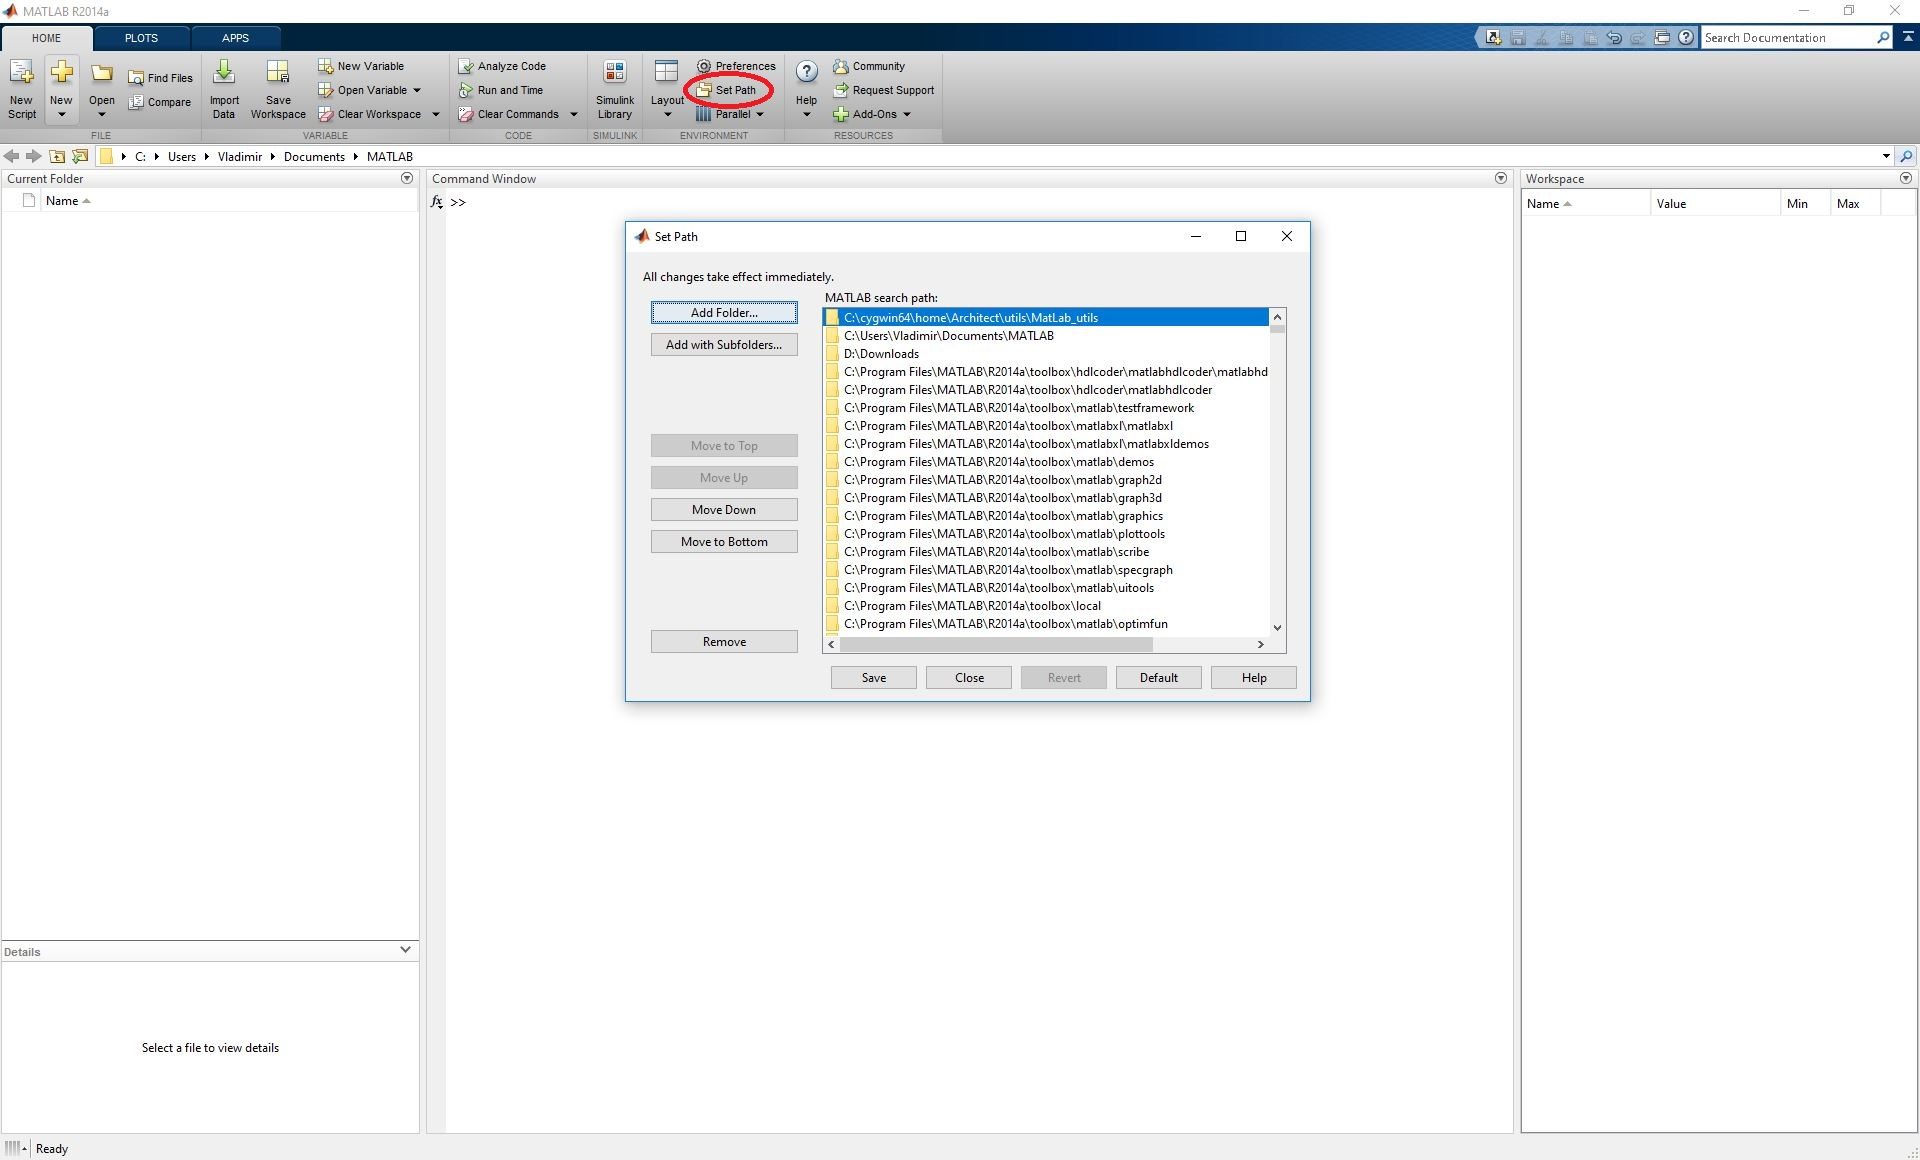
\includegraphics[width=0.6\textwidth]{Set_folder_MathLab.jpg}
\caption{How to add Architect scripts to MatLab.}
\label{fig4}
\end{figure}

In order to use those utilities change the MatLab current folder to the folder where You did ran simulation. The description of those utilities can be found inside ".m" files.









































\end{document}